\documentclass[a4paper,12pt]{article}
\usepackage{fullpage}
\usepackage{enumerate}
\usepackage[T1,T2A]{fontenc}
\usepackage[utf8]{inputenc}
\usepackage[bulgarian]{babel}
\usepackage{graphicx}

\begin{document}

\title{
  Софийски университет ``Св. Климент Охридски''\\
  Факултет по информатика и математика\\
  Индивидуален проект по АПИС
}
\author{}
\date{}

\maketitle

\begin{center}
\begin{tabular}{r|l}
Изготвил & Цветан Цветанов \\
Специалност & Информационни системи \\
Курс & Трети \\
Факултетен номер & 71473 \\
Група & Трета \\
Преподавател & Проф. д-р Калинка Калоянова \\
\end{tabular}
\end{center}

\newpage

\tableofcontents

\newpage

\section{CD модел}

\begin{center}
  \begin{tabular}{ |p{5cm}|p{10cm}| }
    \hline
    \multicolumn{2}{|c|}{\textbf{Намерение}: Потребител желае да потърси обяви по даден критерий.} \\
    \hline
    & \textbf{Тригер}: Потребител натиска бутон ``Търси''. \\
    \hline
    \textbf{Намерение}: Да се намери обява в регион, удобен за потребителя. & Появява се списък с населени места, ако е на мобилно устройство, иначе се появява карта на страната. \\
    \hline
    \textbf{Бележка}: Потребителят може да се върне назад за да поправи критерия. & \\
    \hline
      & Потребителят се препраща към стъпка за избиране на район/квартал. \\
    \hline
    \textbf{Намерение}: Да се намери обява в квартал/район, удобен за потребителя. & Появява се карта на текущо избраното населено място, от която потребителят може да избира квартал/район. Ако е на мобилно устройство се появява само списък. \\
    \hline
    \textbf{Бележка}: Потребителят може да се върне назад за да поправи критерия. & \\
    \hline
     & Потребителят се препраща към стъпка за избиране на характеристики на имота. \\
    \hline
    \textbf{Намерение}: Да се избере имот, който спазва нужните на потребителя характеристики. & Появяват се полета с характеристики, от които потребителят може да избира. Валидно е да се избере повече от една характеристика. \\
    \hline
    \textbf{Бележка}: Потребителят може да се върне назад за да поправи критерия. & \\
    \hline
     & Предоставя се поле за търсене. \\
    \hline
    \textbf{Намерение}: Филтриране на получените резултати чрез търсене в текстовите полета на обявите. & Предоставя се поле за търсене, където потребителят въвежда свободен текст. По този свободен текст се филтрират тези обяви, които го имат в полетата си. \\
    \hline
    \textbf{Бележка}: Потребителят може да се върне назад за да поправи критерия. & \\
    \hline
    \textbf{Намерение}: Уведомяване на потребителя за наличните обяви. & Повявява се списък с обявите спазващи горните четири критерия. \\
    \hline
  \end{tabular}
\end{center}

\newpage

\section{Потребителски случаи в пълен формат}

\subsection{Промяна на статуса на обява}

\begin{verbatim}
use case 19: Промяна на статуса на обява
scope: N/A
level: user-goal
primary actor: Брокер, Администратор
stackeholders & interesets:
  - Брокер: Желае да няма неактуални обяви в системата.
  - Купувачи: Желаят да имат актуална информация в системата, за да не си
      губят времето с "изпуснати" обяви или възможно най-бързо да намерят нова
      обява.
  - Продавачи: Желаят да не получават телефонни обаждания след като са продали
      обявата си. Желаят възможно най-бързо да публикуват имота си. Също така, 
      желаят да имат възможност за промотиране на имотите си.
  - Администратор: Желае системата да е изрядна, в частност, да са актуални
      обявите на някой брокер, дори когато той отсъства.

trigger: Брокер/Администратор избира опция за промяна на статуса на обява

preconditions:
  - Потребителят е в системата като Брокер или Администратор
  - Ако потребителят е Брокер, той може да променя само свои обяви

postconditions:
  - Ако обявата е била Активна, тя е станала Неактивна
  - Ако обявата е била Неактивна, тя е станала Активна
  - Ако обявата е била VIP, тя е станала не-VIP
  - Ако обявата е била не-VIP, тя е станала VIP
  - Ако обявата е Активна, тя се вижда от всички потребители
  - Ако обявата е Неактивна, тя се вижда само от Брокер и Администратор
  - Ако обявата е VIP, тя получава специална наредба в показването на обяви

main success scenario:
  1. Брокер/Администратор избира опция за промяна на статуса на обява
  2. БА избира обявата, чиито статус иска да промени
  3. Системата показва обявата
  4. БА избира новия статус
  5. БА потвърждава избора си
  6. Системата обновява статуса на обявата
  7. Системата записва събитието в одит лога

extensions:
  3a. Няма такава обява
    1. Системата извежда информация за грешка на БА

  4a. Администратор е променил обявата малко преди показването
    1. Системата извежда информативно съобщение
    2. БА го приема
    3. Системата продължава по главния сценарий

  6a. БА не потвърждава избора си
    1. Системата отново показва обявата

  7а. Администратор е променил обявата малко преди обновяването
    1. Системата извежда информативно съобщение
    2. БА го приема
    3. Системата показва обновената от другия БА обява
    4. Системата се връща в точка 5 от главния сценарий

special requirements:
  N/A

frequency of occurrence:
  Около 10-15 пъти в седмица.

други:
  N/A
\end{verbatim}

\subsection{Рейтване на брокер}

\begin{verbatim}
use case 8: Рейтване на брокер
scope: N/A
level: subfunction
primary actor: Регистриран потребител
stackeholders & interesets:
  - Потребител: Да работи с коректни брокери.
  - Брокер: Да има система за поощрение на базата, на която да се гради
      доверие от страна на потребителите.

preconditions:
	- Потребителят се е логнал
  - Потребителят не е рейтвал преди брокера

postconditions:
	- Брокерът има обновен спрямо "хубава" формула рейтинг

main success scenario:
	1. Потребител желае да рейтне брокер
	2. Потребител намира желания брокер
  3. Системата показва профила на брокера
  4. Потребителят избира рейтинг
  5. Потребителят потвърждава рейтинга си
  6. Системата преизчислява рейтинга на брокера
  7. Системата запазва новия рейтинг
  8. Системата предоставя потребителя със съобщение за успех

extensions:
  4a. Рейтингът е извън допустимите граници
    1. Системата показва съобщение за грешка
    2. Потребителят го приема
    3. Системата връща потребителя в точка 4 от главния сценарий

special requirements:
  - Да се използва формула за рейтинг, правеща трудна злоупотребите с
      рейтването на брокери

frequency of occurrence:
  Почти след всяка сделка с брокер.

други:
  N/A
\end{verbatim}

\newpage

\section{Диаграма на взаимодействието}

Следната диаграма показва взаимодействието на потребителя със системата по време на търсене на обяви. \\

При търсене, потребителят трябва да мине през няколко етапа.  Те са описани в
наличната диаграма.  Системата за потребителски интерфейс представлява 
абстрактен изглед на наличните за потребителя способи за контролиране на
минаването през тези етапи.

Резултатите от етапите се акумулират във Филтър, чиято крайна цел е, след
сдобиване с достатъчно информация, да попълни Списъка с обяви, от които
потребителя да си избере нужната обява.

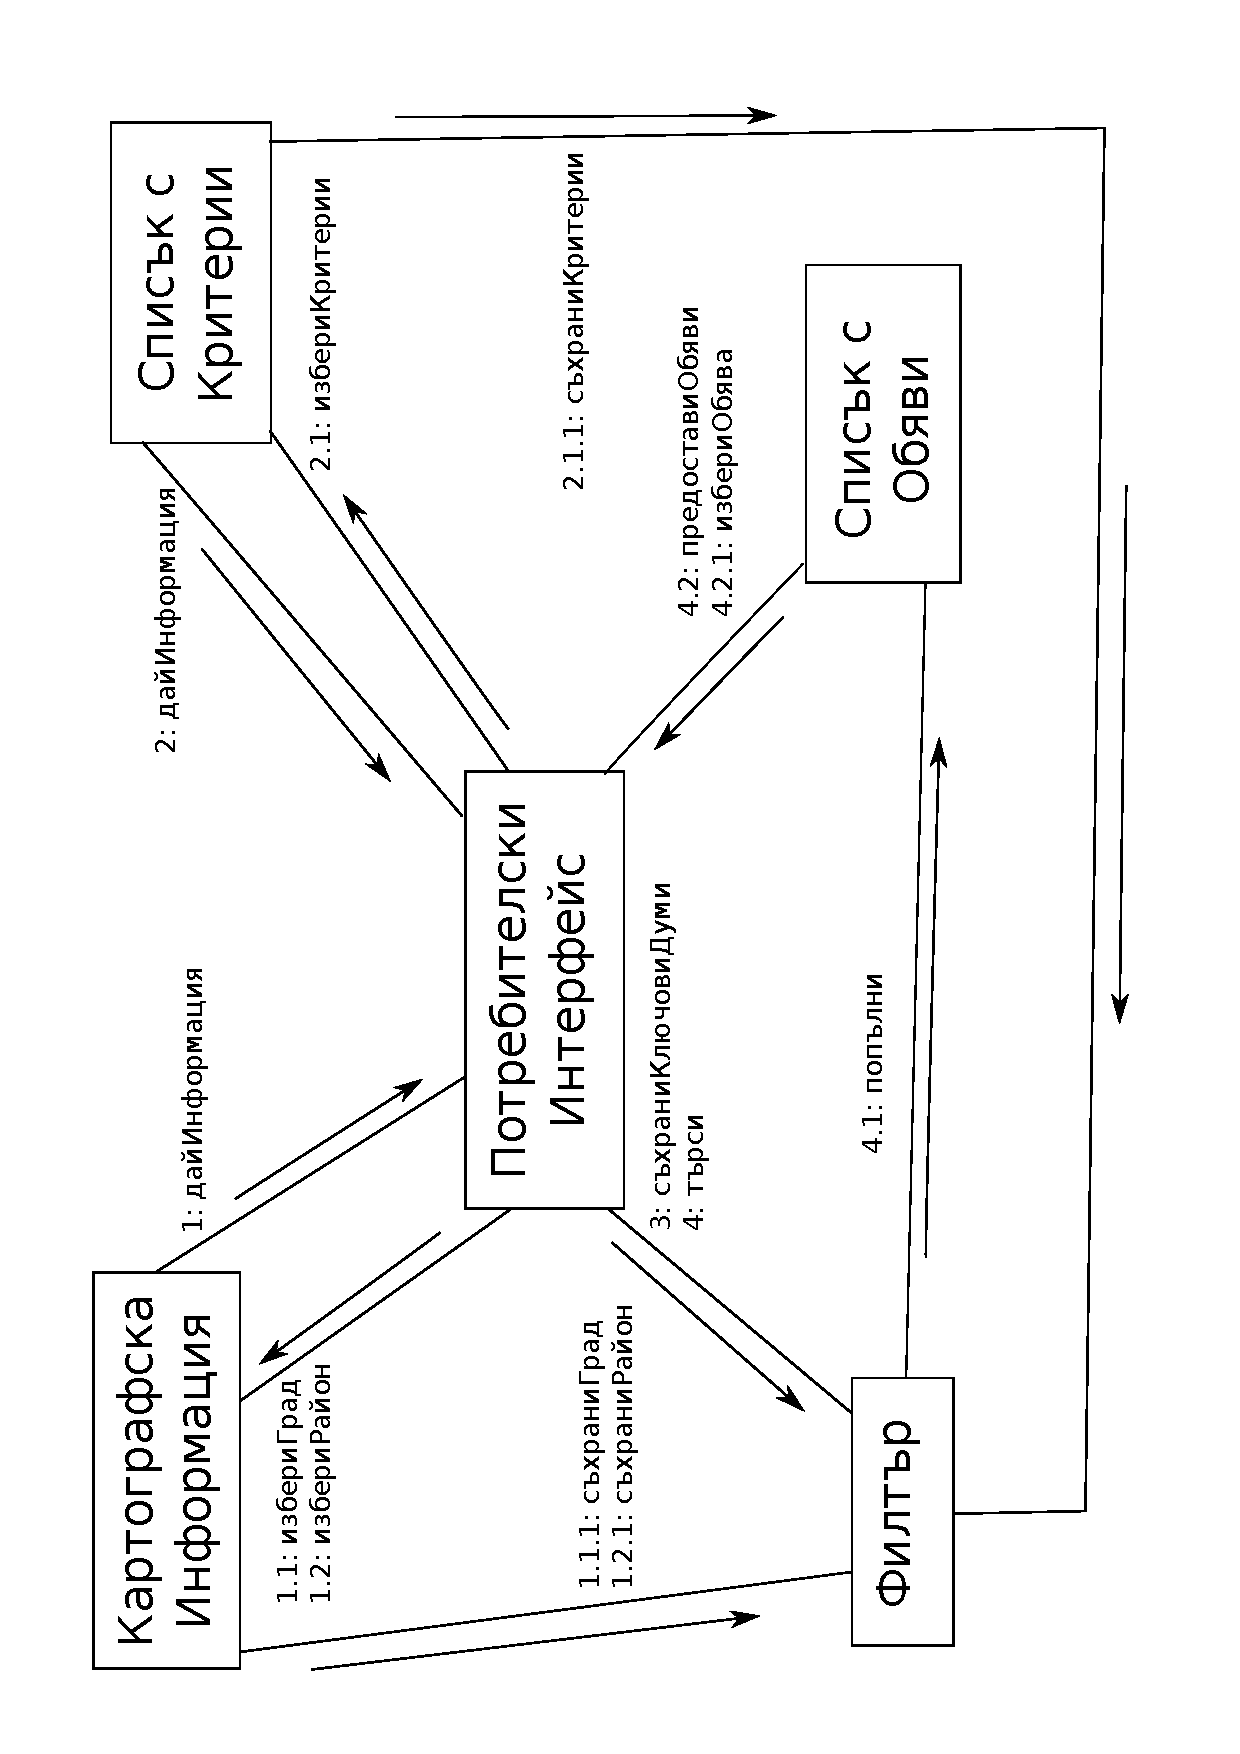
\includegraphics[scale=0.5,keepaspectratio=true]{uml02.pdf}

\end{document}
